\section{Vector Algebra}

\subsection{Vector Magnitude}

\begin{definition}[Vector Magnitude]
  Let $\vec{v} = (v_1, v_2, v_3)$ be a vector in $\mathbb{E}^3$. The \textbf{magnitude} of $\vec{v}$ is defined as:
  \begin{equation}
    \|\vec{v}\| = \sqrt{v_1^2 + v_2^2 + v_3^2}
  \end{equation}
\end{definition}

\subsection{Vector Addition}

\begin{definition}[Vector Addition]
  Let $\vec{v} = (v_1, v_2, v_3)$ and $\vec{w} = (w_1, w_2, w_3)$ be vectors in $\mathbb{E}^3$. The \textbf{sum} of $\vec{v}$ and $\vec{w}$ is defined as:
  \begin{equation}
    \vec{v} + \vec{w} = (v_1 + w_1, v_2 + w_2, v_3 + w_3)
  \end{equation}
\end{definition}

Geometrically this can be seen as the {\bf diagonal} of a paralleleogram. Geometrically it is clear that you get the same effect as travelling along $\vec{v}$ and then $\vec{u}$

\begin{figure}[H]
\centering
   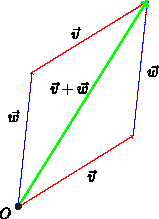
\includegraphics[scale=2.0]{vector_addition.pdf}
   \caption{Vector Addition} 
   \label{fig:figure-2-vector-addition}
\end{figure}

\clearpage

\subsubsection*{Vector Addition Properties}
\vspace{5px}
 
\begin{theorem}[Commutativity]
Suppose $\vec{v}$ and $\vec{w}$ be vectors in $\mathbb{E}^3$.\\
  If $\vec{v} = \left( v_1, v_2, v_3 \right)$ and $\vec{w} = \left(w_1, w_2, w_3 \right)$ be vectors in $\mathbb{E}^{3}$, then
  \begin{equation}
      \vec{v} + \vec{w} = \vec{w} + \vec{v}    
  \end{equation}
\end{theorem}
\begin{proof}
  
\end{proof}

